\documentclass{beamer}

\usepackage{amsmath}
\usepackage{amssymb}
\usepackage{amsthm}
\usepackage[UKenglish]{babel}
\usepackage{enumerate}
\usepackage{graphicx}
\usepackage{braket}
\usepackage{esint}
\usepackage{float}
\usepackage{tabularx}
\usepackage{array}
\usepackage{subcaption}
\usepackage{hyperref}
\hypersetup{colorlinks=false, bookmarks=true}

\usetheme{Madrid}
\usecolortheme{seahorse}
\usefonttheme{professionalfonts}
\useinnertheme{circles}

\AtBeginSection[]
{
  \begin{frame}
    \frametitle{Table of Contents}
    \tableofcontents[currentsection]
  \end{frame}
}

\setbeamertemplate{caption}[numbered]

\title[PQC Function Evaluation]{PQC Function Evaluation}
\subtitle{Carnegie Vacation Scholarship}
\author[David Amorim]{David Amorim}
\institute[]{}
\date[29/07/2024]{Week 4 \\(22/07/2024 - 26/07/2024)}

\begin{document}

\frame{\titlepage}

\begin{frame}
\frametitle{Aims for the Week}
The following aims were set at the last meeting (22/07/2024):

\begin{alertblock}{1. Change Input Layer Structure}
Improve the connectivity of input layers. Each input qubit should ideally control each target qubit at some point in the network. 
\end{alertblock}

\begin{alertblock}{2. Fix Parameters}
Add the option to keep parameters fixed for each type of network layer. 
\end{alertblock}

\begin{alertblock}{3. Improve Loss Function}
Develop a distance measure taking into account digital encoding. Either incorporate this into weights for an existing loss function or define a new loss function on this basis. 
\end{alertblock}
\end{frame}

\begin{frame}
\frametitle{Glossary}
\begin{table}
\begin{center}
\begin{tabularx}{\textwidth}{ c|>{\centering}X}
  \textbf{Acronym} & \textbf{Meaning} \tabularnewline
  \hline 
  CL  & convolutional layer   \tabularnewline
  AA-CL  & all-to-all convolutional layer \tabularnewline
  NN-CL  & neighbour-to-neighbour convolutional layer \tabularnewline
  IL & input layer \tabularnewline 
  SAM & sign-adjusted mismatch
\end{tabularx}
\caption{Acronyms and short-hands used in the following.}
\end{center}
\end{table}
\begin{table}
\begin{center}
\begin{tabularx}{\textwidth}{>{$}c<{$}|>{\centering}X}
  \textbf{Variable} & \textbf{Meaning} \tabularnewline
  \hline 
  n  & input register size   \tabularnewline
  m  &  target register size \tabularnewline
  L  & number of network layers \tabularnewline
\end{tabularx}
\caption{Variables used in the following.}
\end{center}
\end{table}
\end{frame}


\section{Changing Input Layer Structure}

\begin{frame}
\frametitle{Changing Input Layer Structure}
\begin{itemize}
\item Previously, the $j$th input qubit controlled an operation on the $j$th target qubit (with wrap-around for $n >m$) 
\item An optional \alert{shift parameter}, $s$, has now been added so that the $j$th input qubit controls an operation on the $j+s$th target qubit 
\item This shift parameter is incremented for each successive IL 
\item The QCNN is padded with additional ILs to ensure that the number of ILs is $\geq m$ 
\item Thus, \alert{each input qubit now controls an operation on each target qubit} at some point in the QCNN 
\item Note that ILs still alternate between control states 0 and 1
\end{itemize}.
\end{frame}

\begin{frame}
\frametitle{Changing Input Layer Structure}
\begin{columns}
\begin{column}{0.5\textwidth}
\begin{figure}
\centering 
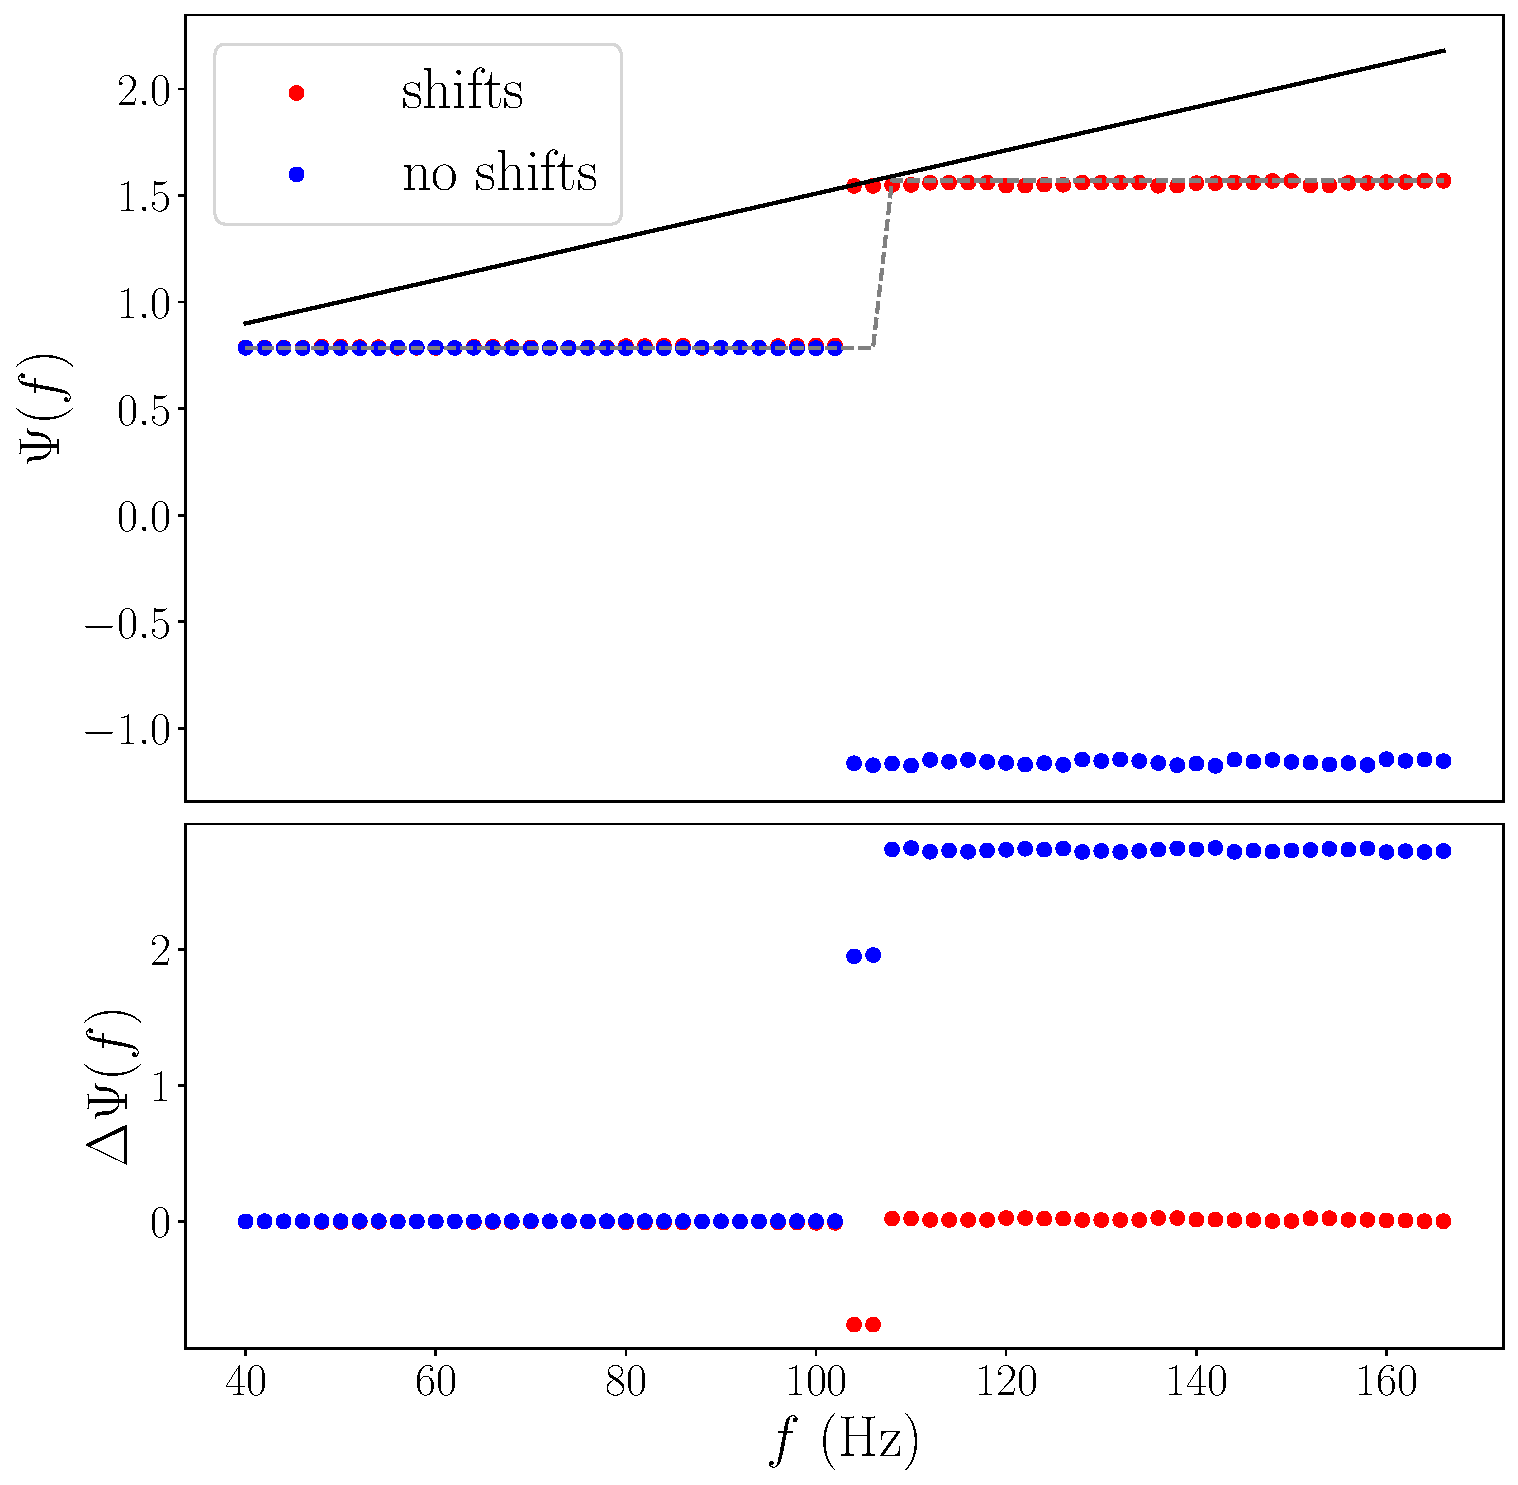
\includegraphics[width=\textwidth]{im/phase_shift_comp_linear_m3}
\caption{Effects of shifted ILs for $\Psi(f) \sim f$ and $m=3$ ($L=6$, 600 epochs, SAM)}
\end{figure}
\end{column}
\begin{column}{0.5\textwidth}
\begin{figure}
\centering 
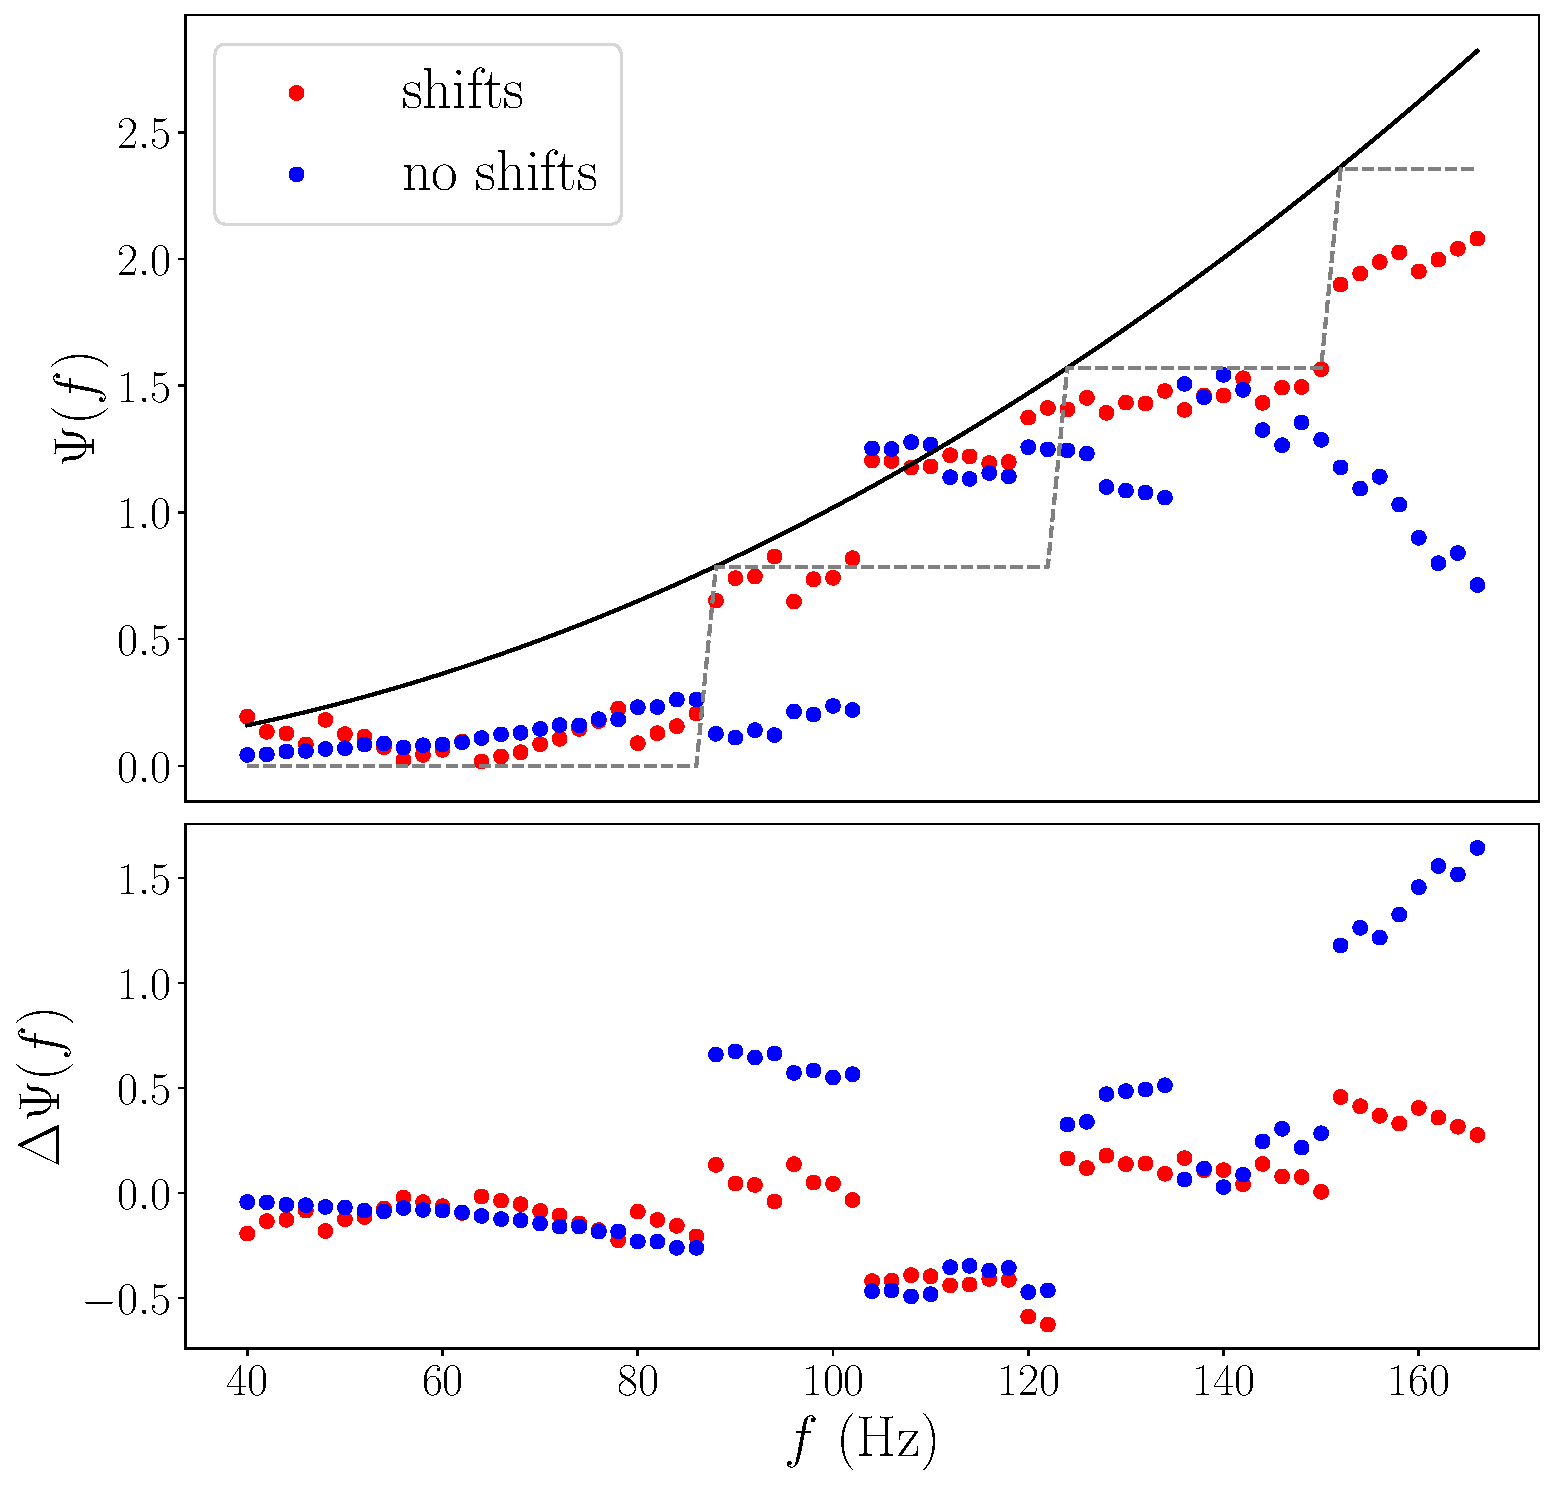
\includegraphics[width=\textwidth]{im/phase_shift_comp_quadratic_m3}
\caption{Effects of shifted ILs for $\Psi(f) \sim f^2$ and $m=3$ ($L=6$, 600 epochs, SAM)}
\end{figure}
\end{column}
\end{columns}
\end{frame}

\begin{frame}
\frametitle{Changing Input Layer Structure}
\begin{columns}
\begin{column}{0.5\textwidth}
\begin{figure}
\centering 
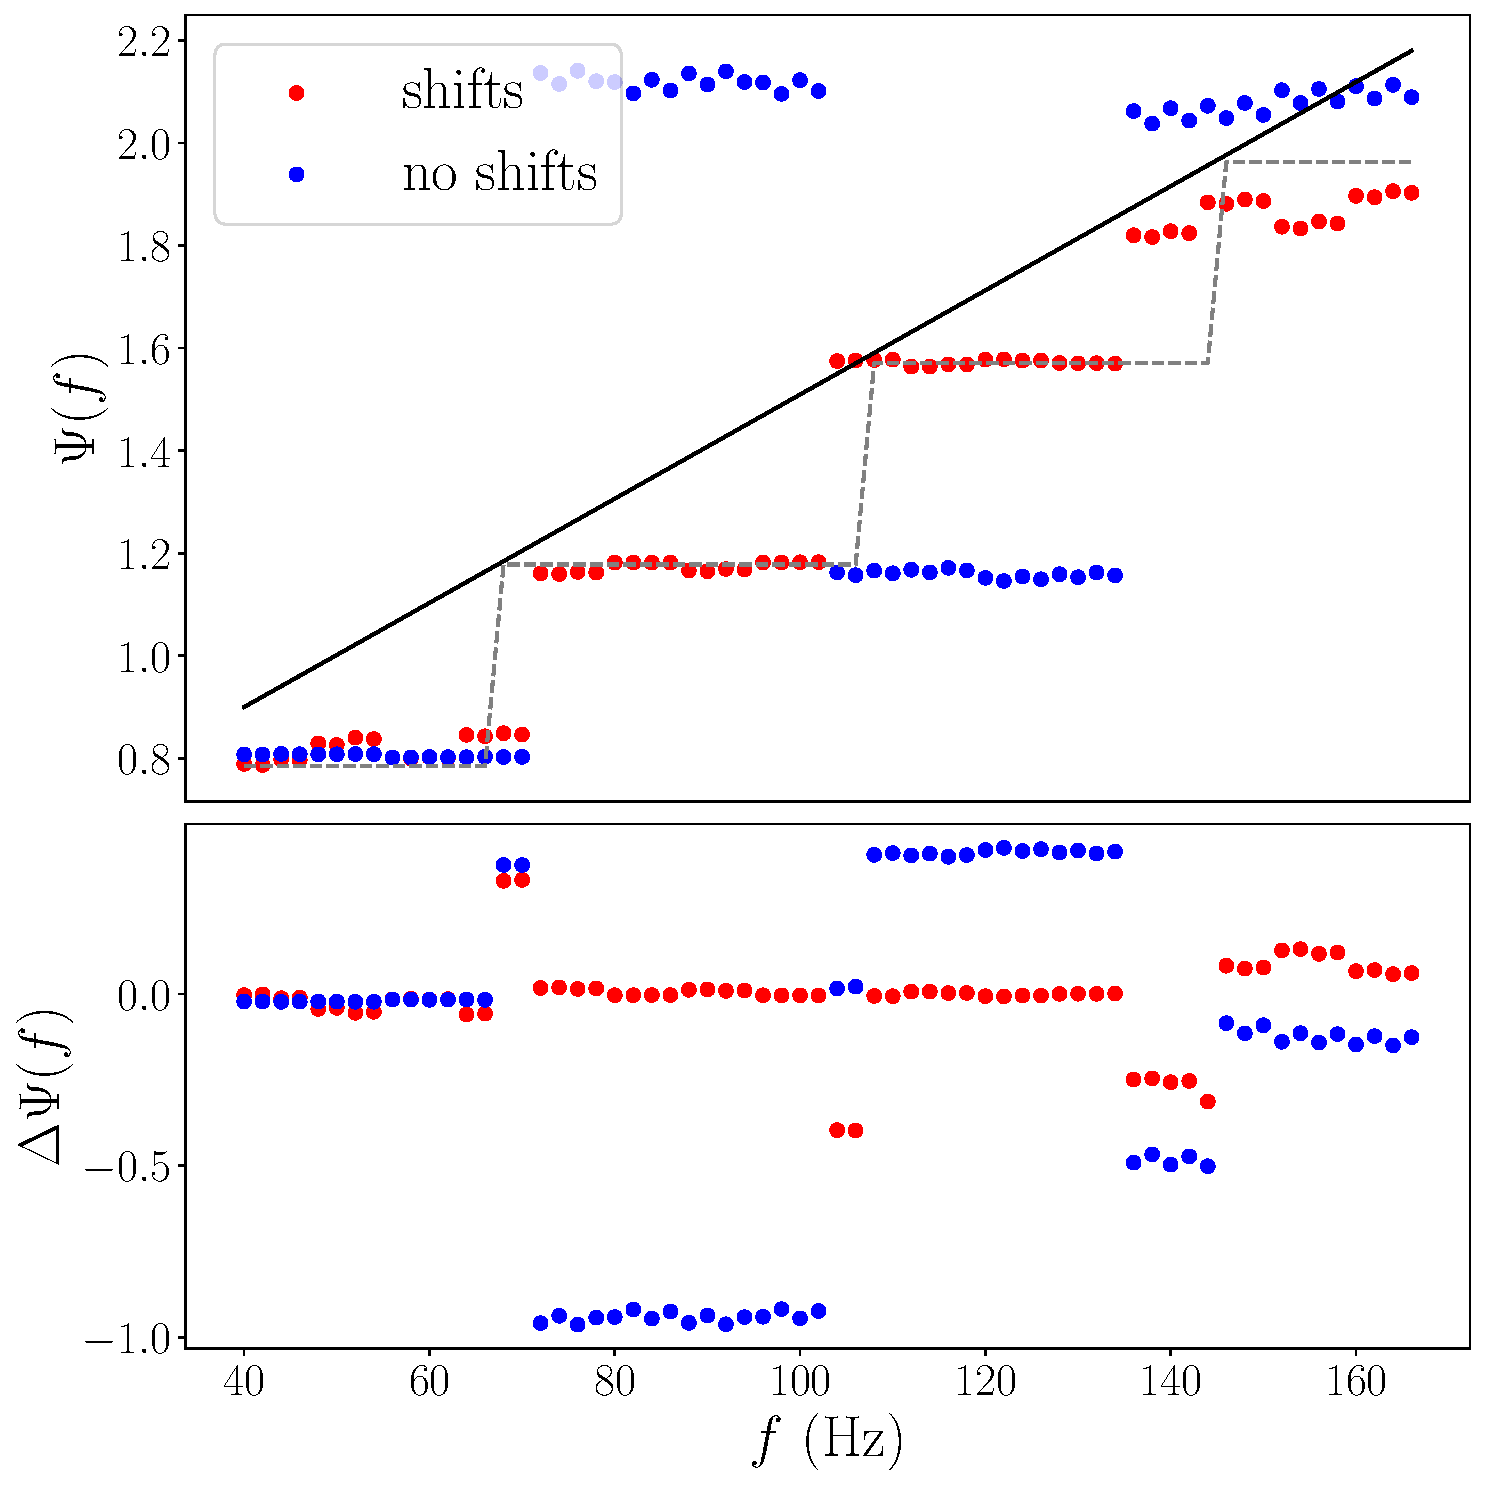
\includegraphics[width=\textwidth]{im/phase_shift_comp_linear_m4}
\caption{Effects of shifted ILs for $\Psi(f) \sim f$ and $m=4$ ($L=6$, 600 epochs, SAM)}
\end{figure}
\end{column}
\begin{column}{0.5\textwidth}
\begin{figure}
\centering 
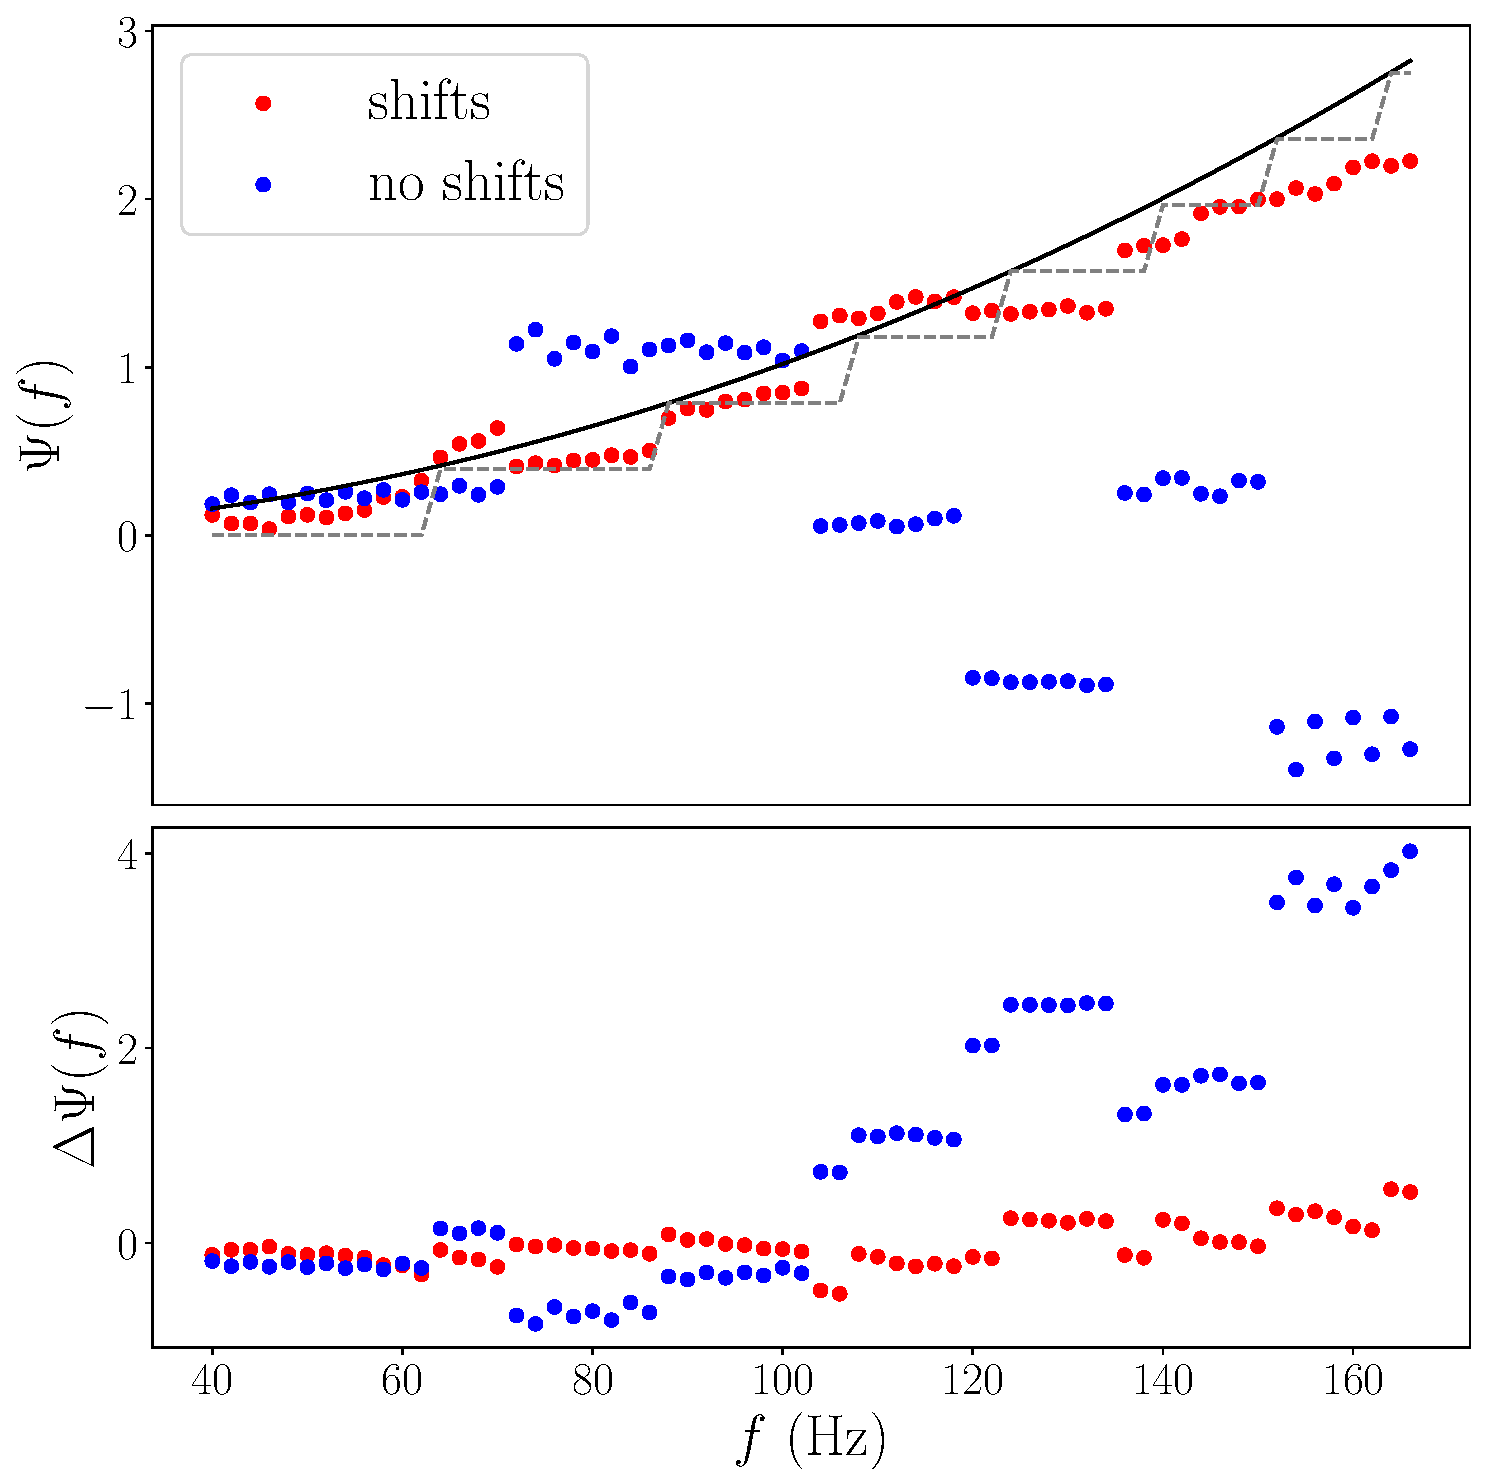
\includegraphics[width=\textwidth]{im/phase_shift_comp_quadratic_m4}
\caption{Effects of shifted ILs for $\Psi(f) \sim f^2$ and $m=4$ ($L=6$, 600 epochs, SAM)}
\end{figure}
\end{column}
\end{columns}
\end{frame}

\begin{frame}
\frametitle{Changing Input Layer Structure}
\begin{columns}
\begin{column}{0.5\textwidth}
\begin{itemize}
\item The data for `no shifts' was obtained by setting  $s=0$ for all ILs instead of incrementing $s$
\item This should be equivalent to last week's circuit structure 
\item However, the `no shifts' results are significantly worse than the results shown last week (\alert{???})
\item Thus, the improvements due to the new IL structure are somewhat exaggerated  
\item Nonetheless, \alert{increased IL connectivity clearly leads to improved performance}
\end{itemize}
\end{column}
\begin{column}{0.5\textwidth}
\begin{figure}
\centering 
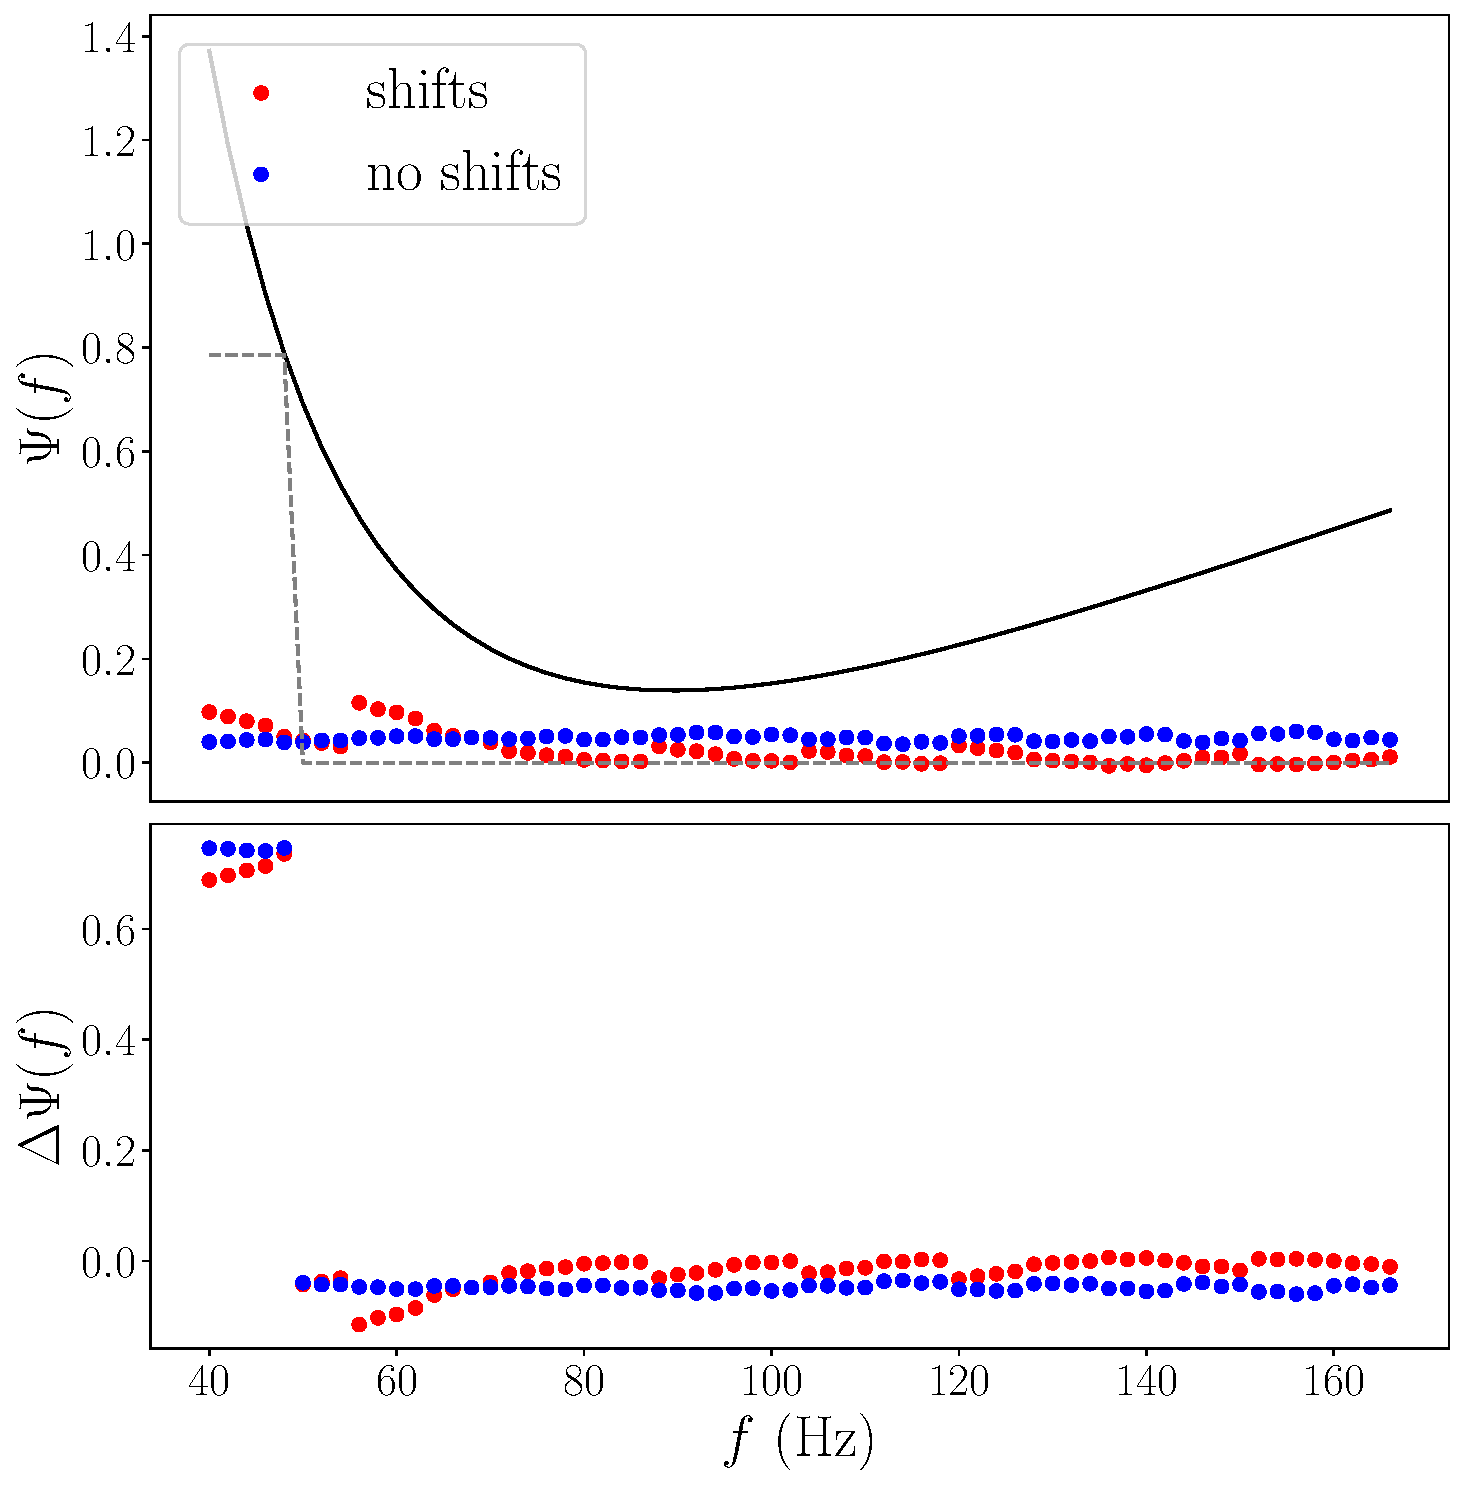
\includegraphics[width=\textwidth]{im/phase_shift_comp_psi_m3}
\caption{Effects of shifted ILs for $\Psi_\text{Hayes2023}$ and $m=3$ ($L=6$, 600 epochs, SAM)}
\end{figure}
\end{column}
\end{columns}
\end{frame}


\section{Fixing Parameters}

\begin{frame}
\frametitle{Fixing Parameters}
\begin{itemize}
\item Implemented the option to \alert{fix parameters for each layer type}
\item This means that each instance of a layer type (IL, AA-CL, NN-CL) uses the same set of parameters 
\item This significantly \alert{reduces the number of trainable parameters} at large $L$
\item Surprisingly, reducing the parameter space \alert{produces no noticeable speed-up} (so-called qiskit primitives, i.e. the sampler, take up roughly 95\% of the computational time)
\end{itemize}
\end{frame}

\begin{frame}
\frametitle{Fixing Parameters}
\begin{columns}
\begin{column}{0.5\textwidth}
\begin{figure}
\centering 
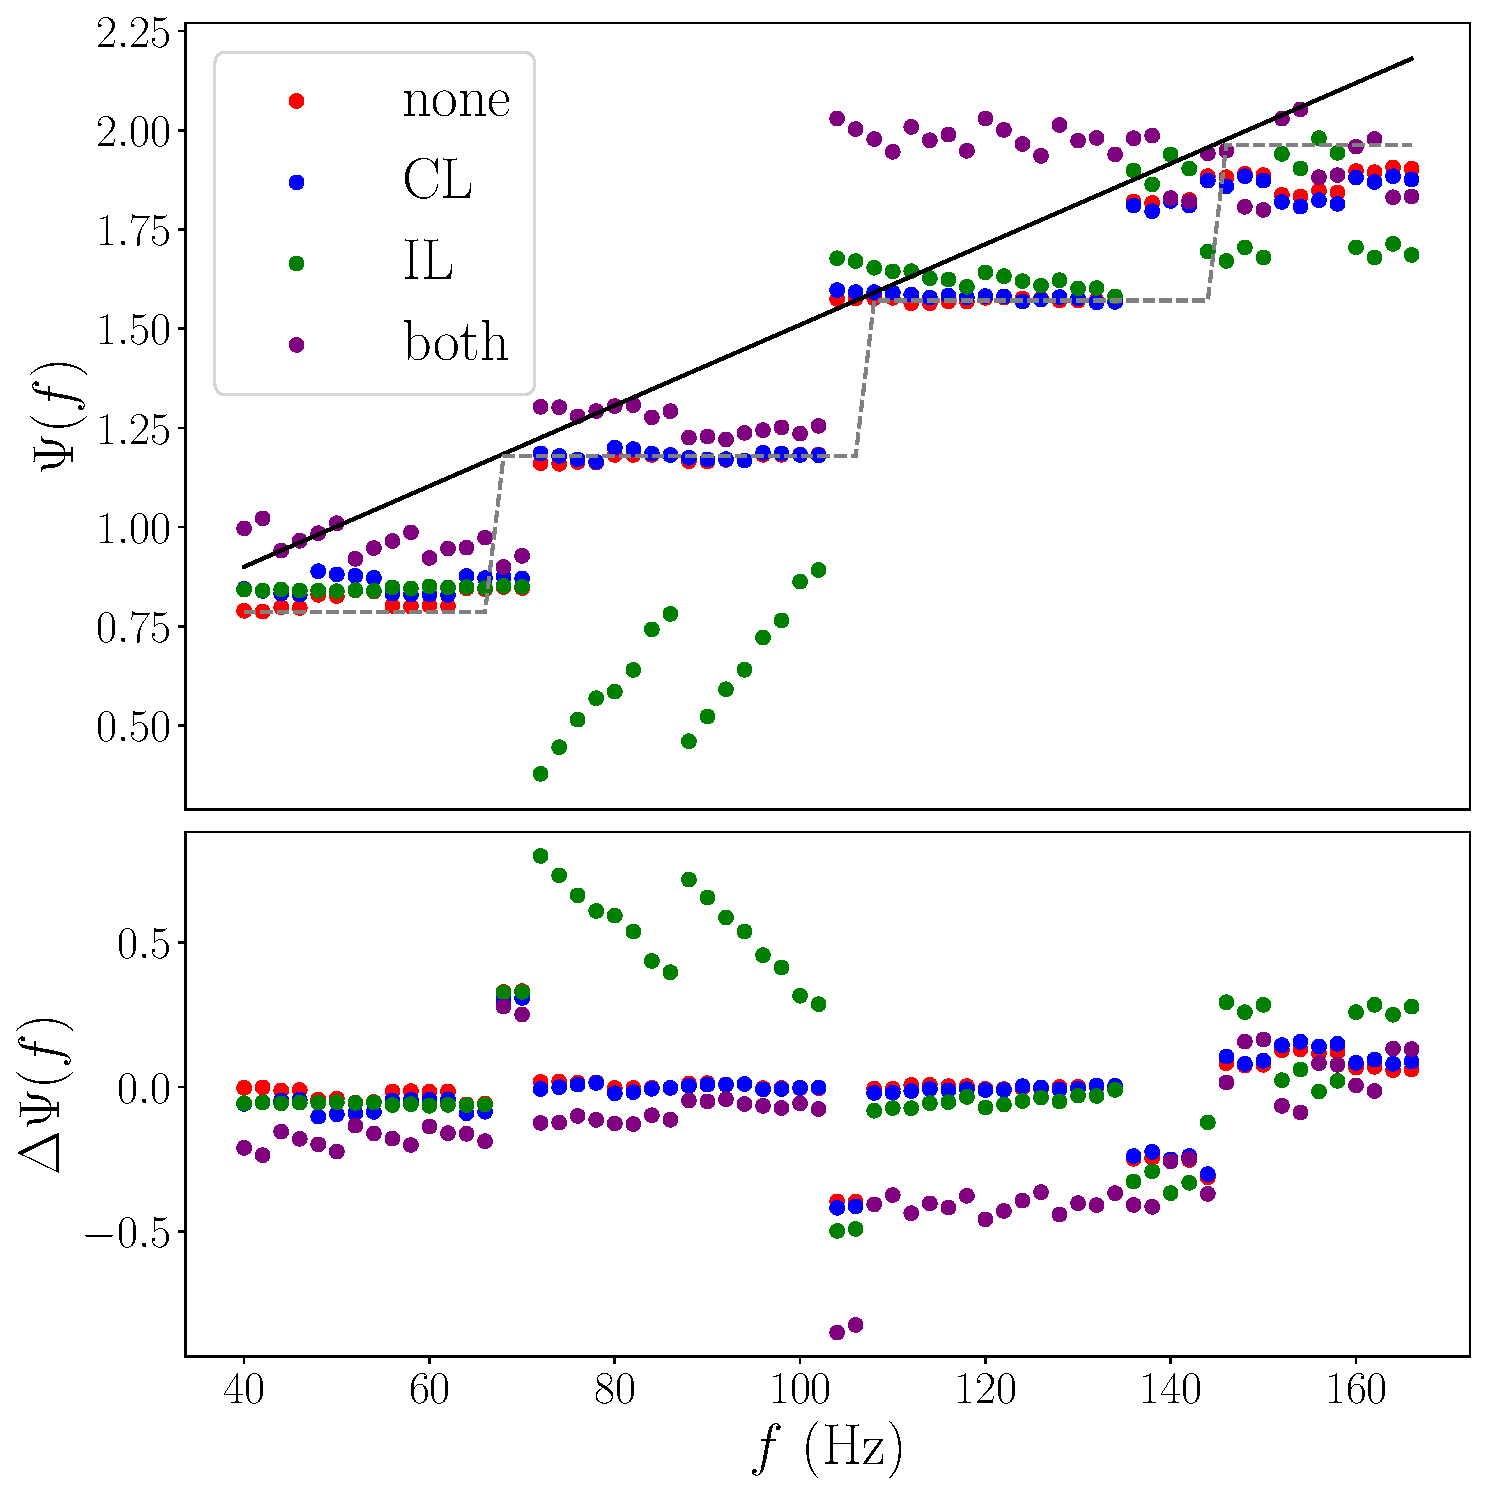
\includegraphics[width=\textwidth]{im/phase_RP_comp_linear_m4}
\caption{Effects of fixing parameters ILs for $\Psi(f) \sim f$ and $m=4$ ($L=6$, 600 epochs, SAM)}
\end{figure}
\end{column}
\begin{column}{0.5\textwidth}
\begin{figure}
\centering 
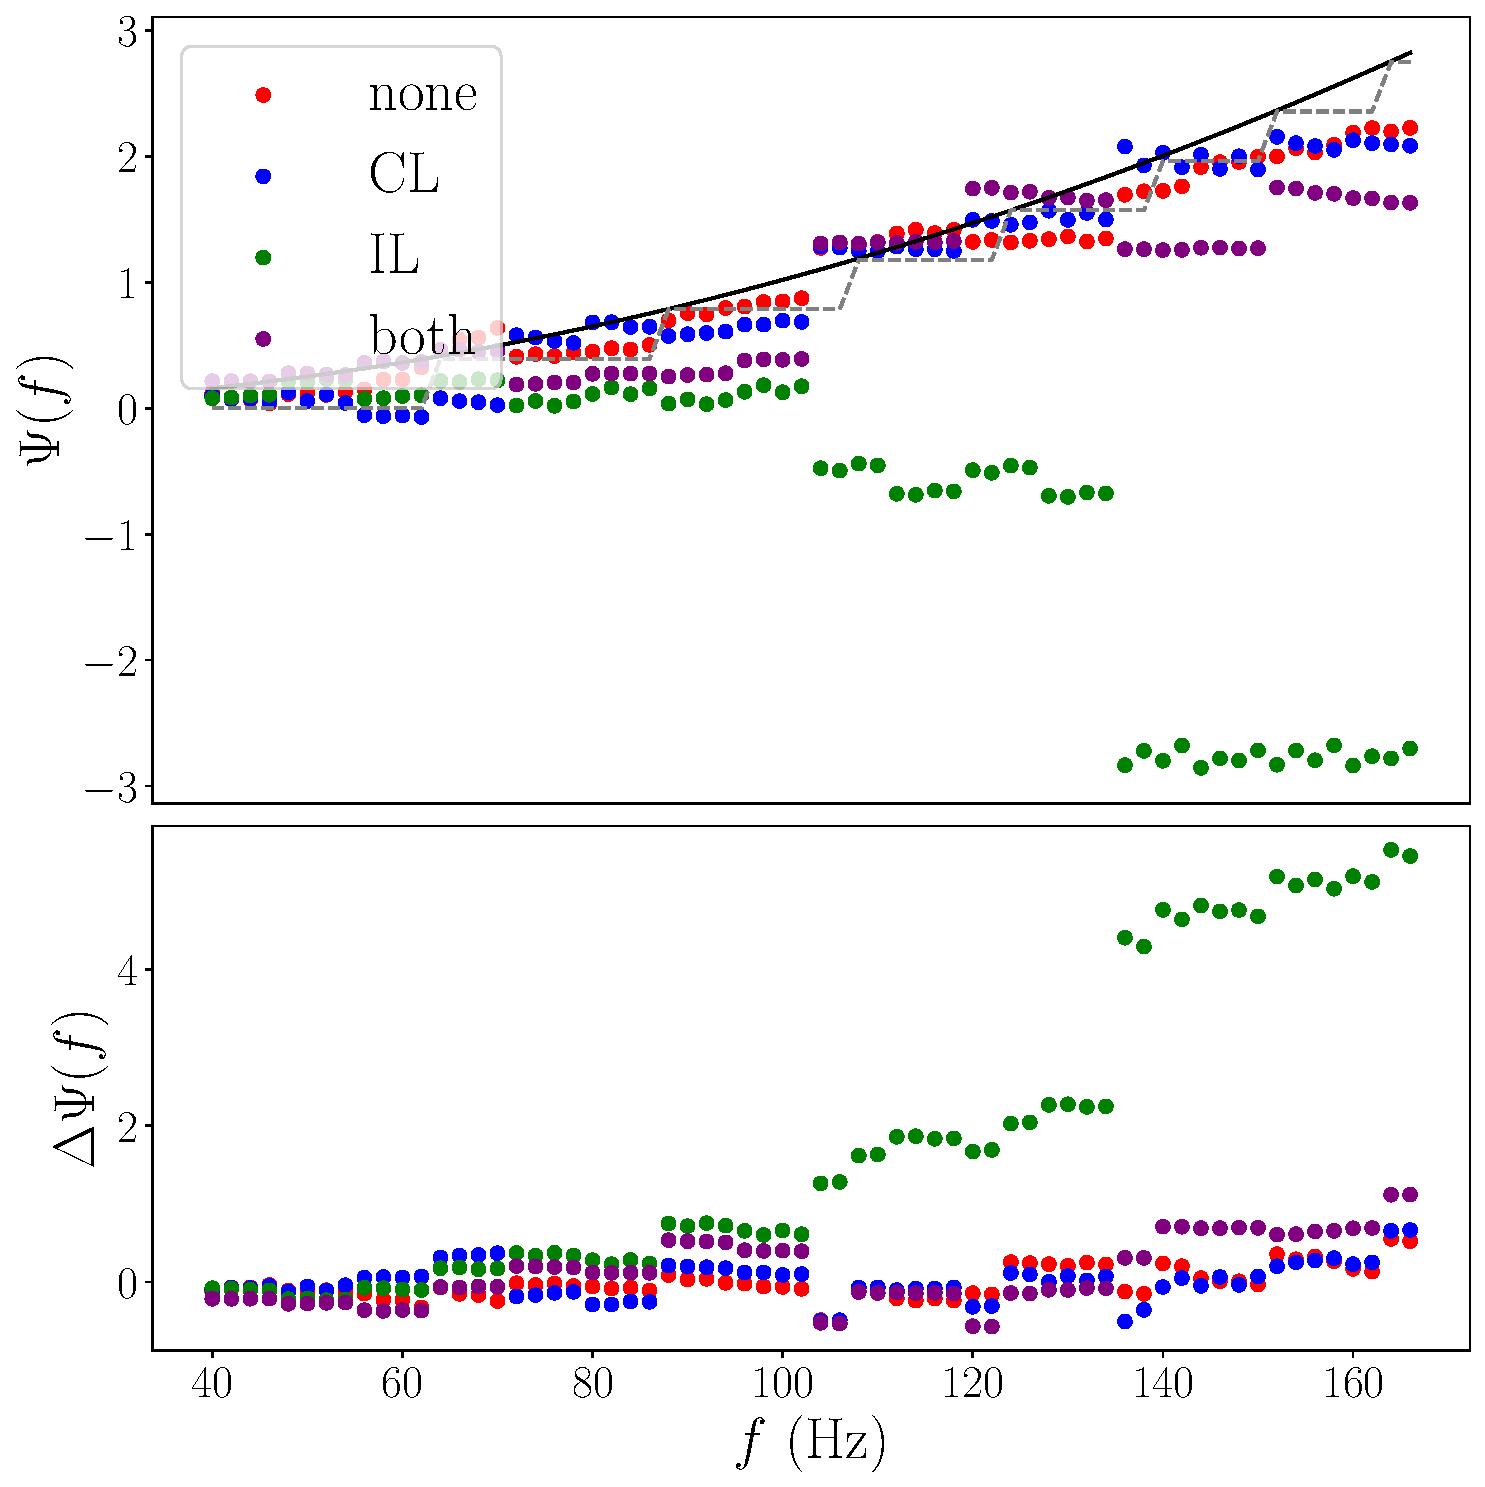
\includegraphics[width=\textwidth]{im/phase_RP_comp_quadratic_m4}
\caption{Effects of fixing parameters for $\Psi(f) \sim f^2$ and $m=4$ ($L=6$, 600 epochs, SAM)}
\end{figure}
\end{column}
\end{columns}
\end{frame}

\begin{frame}
\frametitle{Fixing Parameters}
\begin{itemize}
\item Legend for the plots on the previous slide:
\begin{itemize}
\item `\emph{none}' : no parameters fixed 
\item `\emph{CL}': only CL parameters fixed
\item `\emph{IL}': only IL parameters fixed 
\item `\emph{both}': all parameters fixed  
\end{itemize} 
\item Evidently, keeping parameters fixed leads to (slightly, for `\emph{CL}', or drastically, for `\emph{IL}' and `\emph{both}') \alert{worse performance} 
\item This is likely due to a reduction of the search space 
\item Note that `\emph{IL}' as well as `\emph{both}' lead to \alert{incomplete phase extraction} (formalise this concept!) and hence somewhat meaningless results 
\item Thus, especially taking into account the equivalent computational times, \alert{not keeping parameters fixed yields better results} 
\item These results suggest a particular importance of ILs compared to CLs 
\end{itemize}
\end{frame}

\section{Improving the Loss Function}

\begin{frame}
\frametitle{Preliminary Definitions}
\begin{itemize}
\item Consider a computational basis state, $\ket{k}$, of the \alert{combined} input-register-target-register \alert{system} 
\item The state $\ket{k}$ is associated with a \alert{bit string} $k = \{0,1 \}^{n+m}$
\item Denote by $[k]_n$ and $[k]_m$ the bit strings of length $n$ and $m$, respectively, associated with each of the registers and write their \alert{concatenation} as 
\begin{equation}
k \equiv [k]_n \diamond [k]_m
\end{equation} 
\item A general state of the two-register system is then written as 
\begin{equation}
\ket{z} = \sum^{2^{n+m}-1}_{k=0} z_k \ket{k}
\end{equation}
and referred to via its \alert{coefficients} $z_k$
\end{itemize}
\end{frame}

\begin{frame}
\frametitle{Preliminary Definitions}
\begin{itemize}
\item When training in superposition, the \alert{desired state} of the system is 
\begin{equation}
\ket{y} = \sum_{j=0}^{2^n-1} \frac{1}{\sqrt{2^n}} \ket{j}_i \ket{\Psi(j)}_t,
\end{equation}
where the subscripts $i$ and $t$ indicate basis states of the input and target registers, respectively
\item This state $\ket{y}$ can be written in terms of the \alert{combined basis} $\{ \ket{k} \}$ via 
\begin{equation}
y_k = \begin{cases}
\frac{1}{\sqrt{2^n}}  & \text{if } k=[k]_n \diamond \Psi([k]_n) \\
0 & \text{else} 
\end{cases}
\end{equation}
\item Further denote the \alert{output state} produced by the QCNN by $\ket{x}$, with associated coefficients $x_k$
\end{itemize}
\end{frame}

\begin{frame}
\frametitle{SAM and Beyond}
\begin{itemize}
\item Recall the definition of \alert{SAM}:
\begin{equation}
\text{SAM}(\ket{x}, \ket{y}) = \left\vert 1 - \sum_k x_k y_k \right\vert 
\end{equation}
\item By construction, this is closely related to the \alert{mismatch} 
\begin{equation}
\mathsf{M}(\ket{x}, \ket{y}) = 1 - |\braket{x|y}|
\end{equation}
\item While effective, SAM's \alert{fundamental flaw} is that it does not directly take into account the amplitudes $x_k$ for $k$ where $y_k =0$ (i.e. where $[k]_m \neq \Psi([k]_n)$
\end{itemize}
\end{frame}

\begin{frame}
\frametitle{SAM and Beyond}
\begin{itemize}
\item Consider $k=a$ and $k=b$ with $[k]_m \neq \Psi([k]_n)$ for both and 
\begin{equation}
\Big|[a]_m - \Psi([a]_n) \Big| \geq \Big|[b]_m - \Psi([b]_n) \Big| 
\end{equation}
\item To improve performance, the loss function should punish a non-zero $x_a$ more than a non-zero $x_b$ which is not the case for SAM
\item This could be achieved via a \alert{weighted mismatch}, 
\begin{equation}
\text{WIM}(\ket{x}, \ket{y}) = \left\vert 1 - \sum_k \tilde{w}_k x_k y_k \right\vert, 
\end{equation}
where $\tilde{w}_k \in \mathbb{R}_+$ are appropriate weights
\end{itemize}
\end{frame}

\begin{frame}
\frametitle{SAM and Beyond}
\begin{itemize}
\item It was discussed at the last meeting to base the weights on
\begin{equation}
w_k = \sum^{2^m -1}_{\substack{l=0, \\ l \neq [k]_m}} \Big|x_{[k]_n \diamond l} \Big| \Big| l - \Psi([k]_n) \Big|,
\end{equation}
with the $\tilde{w}_k$ obtained from the $w_k$ via normalisation and smoothing ($\tilde{w}_k \sim e^{\tau w_k}$)
\item Implementing this \alert{proved to be uneffective}, with no improvement on SAM  
\item This raises broader questions about the \alert{feasibility of WIM}
\end{itemize}
\end{frame}

\begin{frame}
\frametitle{The Limits of WIM}
\begin{itemize}
\item SAM is effective as it learns to maximise the $x_k$ for $k$ with $y_k \neq 0$ without regard for the remaining $x_k$
\item It effectively optimises over a \alert{reduced set of states} 
\item This is, presumably, why it outperforms more global loss functions, which directly take into account all coefficients, like L$_1$ loss 
\item Thus, it seems that SAM's \alert{`fundamental flaw'}, of disregarding most $x_k$, is really the \alert{basis of its success} 
\item Adding weights to SAM (WIM) likely is insufficient to alter its fundamental dynamic (or will alter it detrimentally)  
\item Therefore, \alert{WIM will be abandoned for the foreseeable future}
\end{itemize}
\end{frame}

\begin{frame}
\frametitle{Introducing WILL}
\begin{itemize}
\item To improve on SAM, it could be beneficial to return to a loss function, which more directly takes into account all $x_k$ (e.g. L$_1$ loss)
\item More generally, define \alert{L$_\text{p}$ loss} as 
\begin{equation}
\text{LL}_\text{p} (\ket{x}, \ket{y}) = \left( \sum_k |x_k -y_k|^p \right)^{1/p},
\end{equation}
for some $p \geq 1$
\item Note that for phase encoding, \alert{computational basis states are not equidistant}: their distance depends on the value they encode on the input and target registers
\item A \alert{weighted L$_\text{p}$ loss (WILL)} can factor in an appropriate distance measure for the state space:
\begin{equation}
\text{WILL}_\text{p,q} =  \left( \sum_k \Big|x_k -y_k \Big|^p \Big|[k]_m - \Psi([k]_n) \Big|^q \right)^{1/p}
\end{equation}
\end{itemize}
\end{frame}

\begin{frame}
\frametitle{Testing WILL}
\begin{itemize}
\item SPEND SOME TIME PLAYING AROUND WITH p AND q!
\item SEEMS LIKE $q > 1$ makes the MEAN worse but reduces STD! (at least for p=1)  
\item $q=0$ corresponds to L1 

\end{itemize}
\end{frame}


\section{Results}

\begin{frame}
\frametitle{Results}
Show phase encoding with improved methods 
show the full waveform [new frame]
\end{frame}

\section{Next Steps}

\begin{frame}
\frametitle{Next Steps}
\begin{itemize}
\item formalise and investigate `completeness of phase extraction' 
\item look into adding more ILs compared to CLs ?
\end{itemize}
\end{frame}



\end{document}